\documentclass[9pt]{beamer}
%\documentclass[9pt,aspectratio=169]{beamer}
\usepackage[utf8]{inputenc}
\usepackage[english]{babel}
\usepackage[T1]{fontenc}
\usepackage{tikz}
\usepackage{times}
\usefonttheme[onlymath]{serif} 
\usepackage{etoolbox}
\usepackage{xcolor}
\usepackage{amsmath}
\usepackage[absolute,overlay]{textpos}
\usepackage{animate}
\usepackage{booktabs}
\usepackage{verbatim}
\usepackage{biblatex}
\addbibresource{dlpbibli.bib}

% Defining new colors
\definecolor{DarkGreen}{rgb}{0.0, 0.65, 0.31}
\definecolor{NewRed}{rgb}{0.89, 0.02, 0.17}


\usetheme{ARMINES}

\author[Daniella LOPES PINTO]{Daniella LOPES PINTO \textsuperscript{1,2*} \\ 
\texttt{\textcolor{black}{daniella.lopes\_pinto@minesparis.psl.eu}}}
\subtitle{\LARGE Finite element models for the study of hydrogen embrittlement of steel structures}

\institute
{\textbf{Academic advisor}: Jacques BESSON \textsuperscript{1} \\
\vspace{0.25cm}
\textbf{Industrial advisors}: Nikolay OSIPOV \textsuperscript{2} \\
\vspace{0.4cm}
{\textsuperscript{1} Centre des Matériaux, Mines Paris} \\
\vspace{0.15cm}
\textsuperscript{2} Transvalor S.A. \\
\vspace{0.2cm}
\center{\textbf{Thesis defense} \\ \small March 7\textsuperscript{th} 2025} 
\center{\textcolor{white}{XXXXXXXX}}}


\begin{document}

\begin{frame}[plain]
    \maketitle
\end{frame}

%\section{Introduction}
%
%%%%%%%%%%%%%%%%%%%%%%%%%%%%%%%%%%%%%%%%%%%%%%%%%%%%%%%%%%%%
%
%\begin{frame}{Introduction}
%
%    \begin{itemize}
%        \item Item 1
%        \item Item 2
%        \item Item 3
%    \end{itemize}
%
%\end{frame}
%
%%%%%%%%%%%%%%%%%%%%%%%%%%%%%%%%%%%%%%%%%%%%%%%%%%%%%%%%%%%%
%
%\begin{frame}{Outline}
%    \tableofcontents
%\end{frame}
%
%%%%%%%%%%%%%%%%%%%%%%%%%%%%%%%%%%%%%%%%%%%%%%%%%%%%%%%%%%%%

\section{Hydrogen inside metals}

\begin{frame}{Outline}
    \tableofcontents[
        currentsubsection,
        hideothersubsections,
        sectionstyle=show/shaded,
        subsectionstyle=show/shaded,
    ]
\end{frame}

%%%%%%%%%%%%%%%%%%%%%%%%%%%%%%%%%%%%%%%%%%%%%%%%%%%%%%%%%%%

\begin{frame}{Hydrogen uptake}

\begin{itemize}
	\item \textbf{Sieverts' law:} The solubility of a diatomic gas in a metal is proportional to the square root of the gas pressure
\end{itemize}

\vspace{1cm}

    \begin{minipage}{0.55\textwidth}
        \centering
        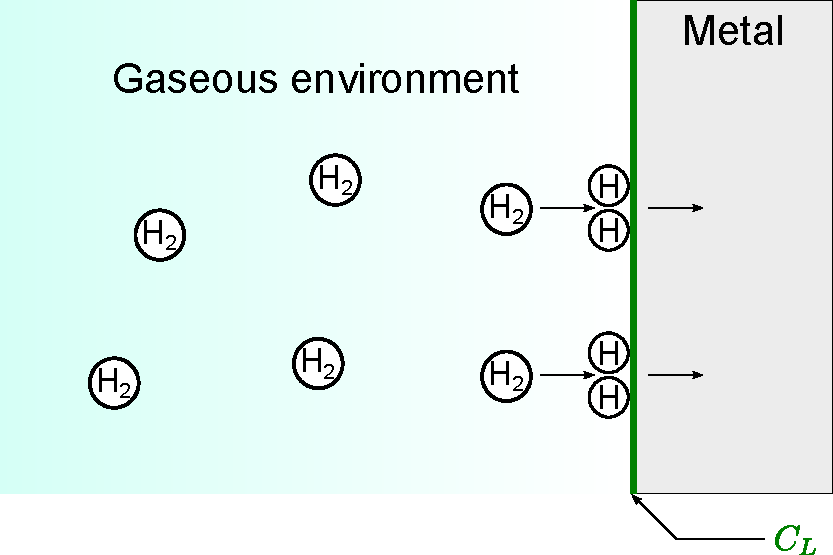
\includegraphics[width=\textwidth]{Images/H2_uptake.pdf}
    \end{minipage}
    \hfill
    \begin{minipage}{0.42\textwidth}
        \centering
        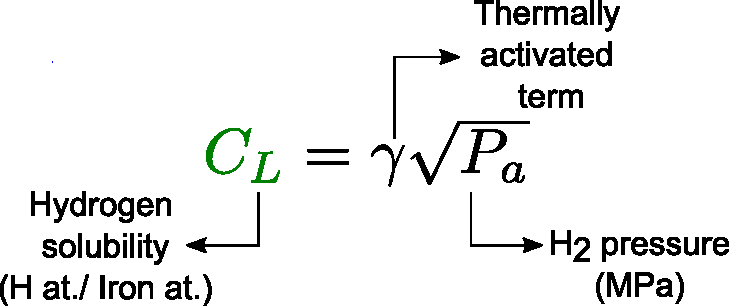
\includegraphics[width=\textwidth]{Images/sieverts.pdf}
    \end{minipage}

\end{frame}

%%%%%%%%%%%%%%%%%%%%%%%%%%%%%%%%%%%%%%%%%%%%%%%%%%%%%%%%%%%

\begin{frame}{Hydrogen diffusion and trapping}

    \begin{columns}
    
        \begin{column}{0.8\textwidth}
    
            \begin{itemize}
                \item Model from \textcolor{darkgray}{Sofronis and McMeeking (1989)} and corrected by \textcolor{darkgray}{Krom \textit{et al.} (1999)}
                
                \vspace{0.35cm}
            
                \item \textbf{Hydrogen concentration:} \hspace{0.5cm} $ \displaystyle C = \textcolor{DarkGreen}{C_L} + \textcolor{blue}{C_T}$
    
                \begin{itemize}
                    \vspace{0.35cm}
                    \item Lattice concentration: \hspace{1.0cm} $\displaystyle \textcolor{DarkGreen}{C_L} = \beta N_L \theta_L$
                    
                    \vspace{0.35cm}
        
                    \item Trapped concentration: \hspace{0.8cm} $\displaystyle \textcolor{blue}{C_T} = \textcolor{NewRed}{N_T(\kappa)} \theta_T$
    
                \end{itemize}
    
                \vspace{0.35cm}
    
                \item \textbf{Hydrogen flux:}
    
                \begin{equation*}
                    J = -D_L \nabla \textcolor{DarkGreen}{C_L} + \frac{D_L \textcolor{DarkGreen}{C_L} V_H}{RT} \textcolor{NewRed}{\nabla P}
                \end{equation*}
            
                \vspace{0.1cm}
            
                \item \textbf{Oriani's equilibrium:}
                
                \begin{equation*}
                    \frac{1- \theta_L}{\theta_L} \frac{\theta_T}{1- \theta_T} = K
                \end{equation*}
                  
            \end{itemize}
    
            \vspace{0.3cm}
            
        \end{column}
        
        \begin{column}{0.2\textwidth}
        \end{column}
        
	\end{columns}
	
	\begin{tikzpicture}[remember picture, overlay]
    	\node at (current page.south west) [xshift=9.5cm, yshift=6cm] {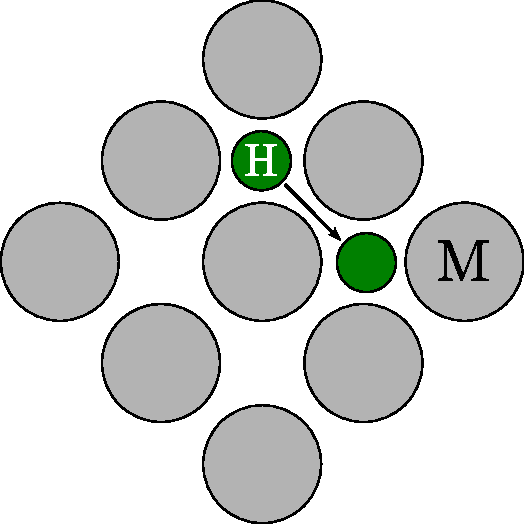
\includegraphics[width=2.5cm]{Images/CL.pdf}}; 
    \end{tikzpicture}
    
    \begin{tikzpicture}[remember picture, overlay]
		\node at (current page.south west) [xshift=10cm, yshift=2.5cm] {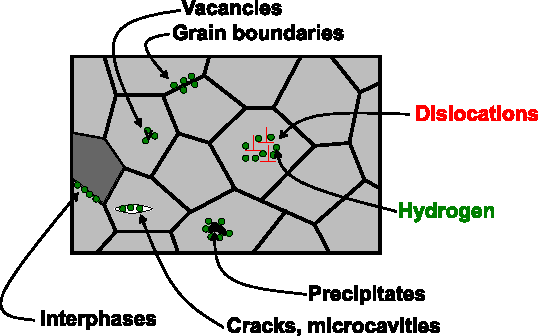
\includegraphics[width=4.5cm]{Images/CT.pdf}}; 
	\end{tikzpicture}
     
	\begin{textblock}{5}(1,14.)
        \textcolor{NewRed}{\footnotesize (Coupling terms)}
    \end{textblock}

\end{frame}

%%%%%%%%%%%%%%%%%%%%%%%%%%%%%%%%%%%%%%%%%%%%%%%%%%%%%%%%%%%

\begin{frame}{Damage}

    \begin{itemize}
        \item The \textbf{ductile behavior} of the metal is described by the \textbf{GTN model} (\textcolor{darkgray}{Tvergaard \textit{et al.} 1984}):
     \end{itemize}

        $$ \displaystyle \frac{\sigma_{eq}^2}{\sigma_F^2} + 2 q_1 f_* \cosh \left(\frac{q_2}{2} \frac{\sigma_{ii}}{\sigma_F}\right) - 1 -q_1^2 f_*^2 = 0 $$ 

        \vspace{0.15cm}

        $$ \displaystyle \dot{f} = \dot{f}_{nucleation} + \dot{f}_{growth} $$

        \vspace{0.15cm}

        \begin{figure}
            \centering
            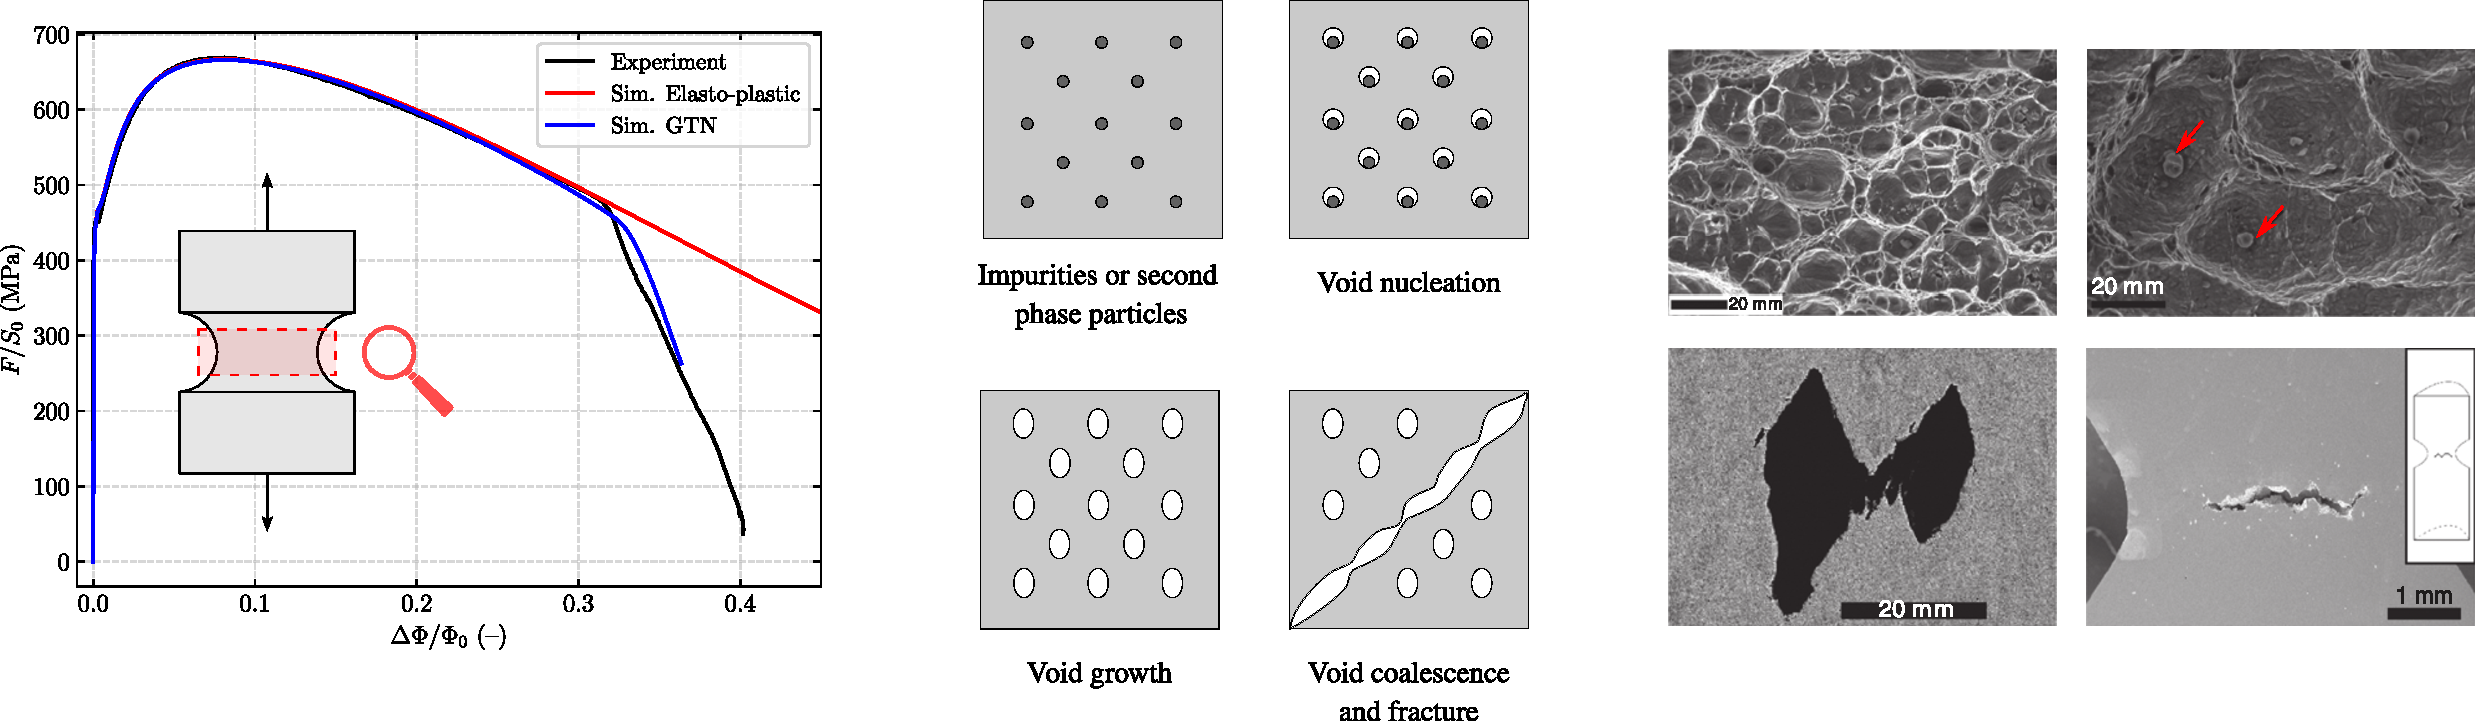
\includegraphics[width=0.98\textwidth]{Images/GTN_sim_exp.pdf}
        \end{figure}
        
\end{frame}

%%%%%%%%%%%%%%%%%%%%%%%%%%%%%%%%%%%%%%%%%%%%%%%%%%%%%%%%%%%

\begin{frame}{Hydrogen embrittlement}

    \begin{itemize}

        \item \textbf{Void growth}: Unchanged due to mass conservation
        
        \begin{equation*}
            \dot{f}_g = (1-f_g) \textrm{trace}(\dot{\varepsilon}_p)
        \end{equation*}  

        \vspace{0.2cm} 
        
        \item\textbf{Void nucleation}: Proposed dependance on hydrogen concentration
        
        \begin{equation*}
            \dot{f}_n = A_n (\kappa) \dot{\kappa} + \textcolor{NewRed}{B_n (C)} \dot{\kappa}
        \end{equation*}

    \end{itemize}
    
    \hspace{1.5cm} 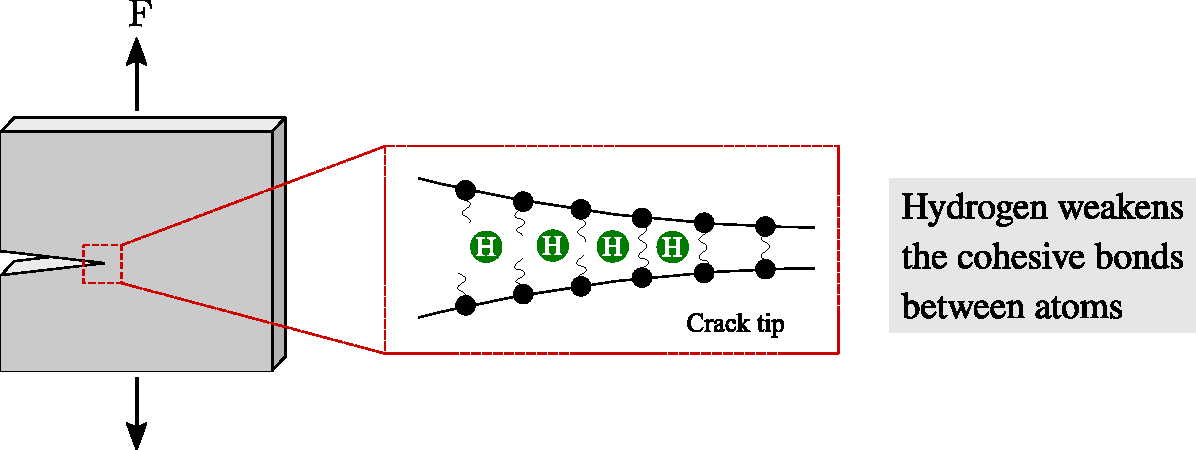
\includegraphics[width=0.75\textwidth]{Images/HEDE3.pdf}

    \begin{textblock}{10}(5,13.5)
        \textcolor{NewRed}{$B_n (C)$}: Damage nucleation due to hydrogen \\ \textbf{HEDE} (Hydrogen Enhanced Decohesion)
    \end{textblock}
    
    \begin{textblock}{5}(13.,7.5)
        \textcolor{NewRed}{\footnotesize (Coupling terms)}
    \end{textblock}

\end{frame}

%%%%%%%%%%%%%%%%%%%%%%%%%%%%%%%%%%%%%%%%%%%%%%%%%%%%%%%%%%%

\section{Finite element formulation}

\begin{frame}{Outline}
    \tableofcontents[
        currentsubsection,
        hideothersubsections,
        sectionstyle=show/shaded,
        subsectionstyle=show/shaded,
    ]
\end{frame}

%%%%%%%%%%%%%%%%%%%%%%%%%%%%%%%%%%%%%%%%%%%%%%%%%%%%%%%%%%%



\begin{frame}{Mixed formulation}

    \begin{itemize}
        \item Fully implicit finite strain framework
        \vspace{0.1cm}
        \item Based on a mixed formulation: $\underline{u}, P, \theta$ (\textcolor{darkgray}{Zhang \textit{et al.} 2017}) and $C_L$ 
        \vspace{0.1cm}
        \item Quadratic elements with reduced integration
        \vspace{0.1cm}
        \item \textbf{Aim:} better pressure fields by avoiding volumetric locking
    \end{itemize}

    \begin{block}{\textbf{Advantage}}
        $\textcolor{NewRed}{\nabla P}$ can be directly computed from nodal values
        \begin{equation*}
            J = {-D_L \nabla C_L} + {{\frac{D_L C_L V_H}{RT} \textcolor{NewRed}{\nabla P}}}
        \end{equation*} 
    \end{block}
    
    \vspace{0.1cm}
    
    \begin{figure}
        \centering
        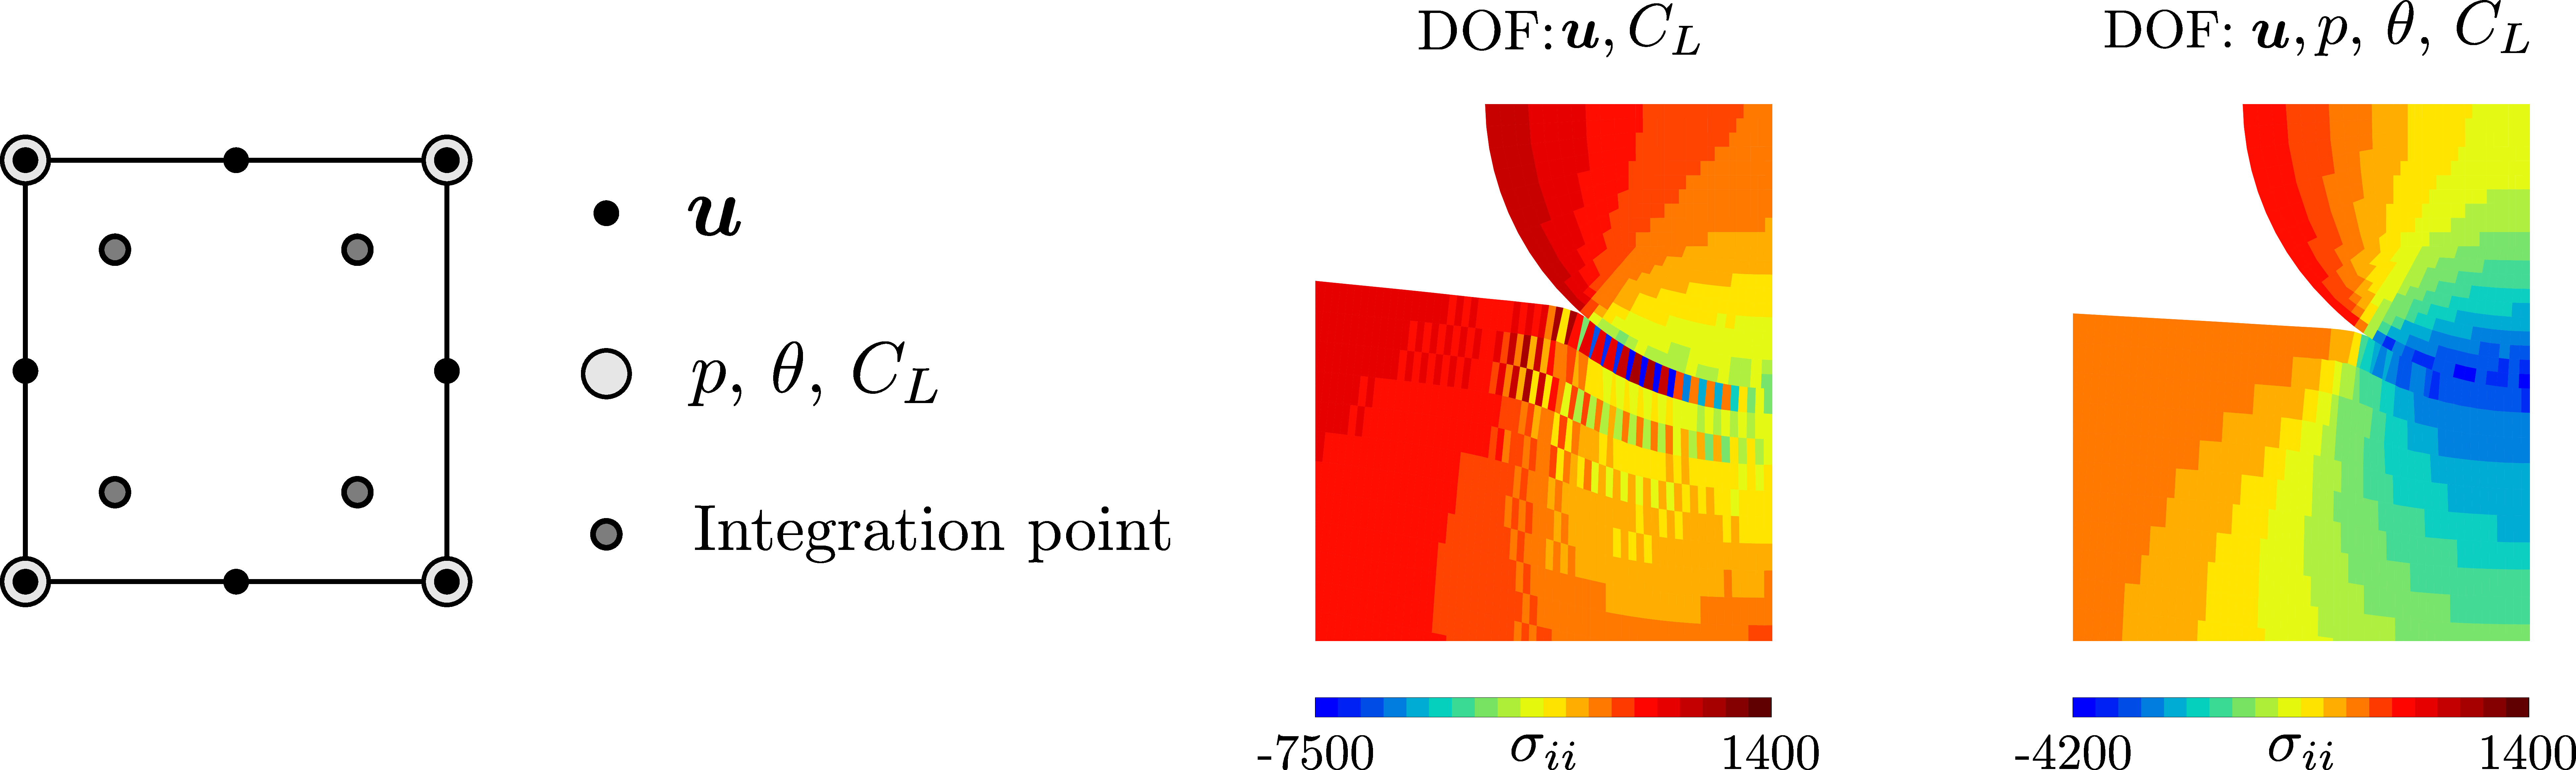
\includegraphics[width=0.9\textwidth]{Images/vol_locking.pdf}
    \end{figure}

    \begin{tikzpicture}[remember picture, overlay]
        \node at (current page.south west) [xshift=11.5cm, yshift=7.5cm] {
\includegraphics[width=2cm]{Images/Zset.jpg}}; 
    \end{tikzpicture}

\end{frame}

%%%%%%%%%%%%%%%%%%%%%%%%%%%%%%%%%%%%%%%%%%%%%%%%%%%%%%%%%%%

\begin{frame}{$B$-bar formulation}
    
	\begin{itemize}
		\item The use of quadratic element lead to high simulation times
		\item $B$-bar formulation: 
	\end{itemize}	    
    
\end{frame}

%%%%%%%%%%%%%%%%%%%%%%%%%%%%%%%%%%%%%%%%%%%%%%%%%%%%%%%%%%%

\section*{}

\begin{frame}{}

    \begin{columns}

        \begin{column}{0.6\textwidth}
            \begin{figure}
                \begin{tabular}{c}
                    
\includegraphics[width=0.6\textwidth]{TEMPLATE_IMAGES/MINES.png} \\
                \end{tabular}
            \end{figure}
        \end{column}

        \begin{column}{0.4\textwidth}
            \begin{figure}
                \begin{tabular}{c}
                    
\includegraphics[width=0.5\textwidth]{TEMPLATE_IMAGES/MESSIAH.pdf} \\
                \end{tabular}
            \end{figure}
        \end{column}

    \end{columns}

    \vspace{0.5cm}

    \noindent\makebox[\linewidth]{\rule{1.0\textwidth}{0.4pt}}

    \vspace{0.3cm}

    \begin{center}
        \Huge{\textcolor{MINESBlue}{\textbf{Thank you for your attention}}} \\
        \vspace{1.0cm}
        \normalsize Daniella LOPES PINTO \\
        \vspace{0.1cm}
        \small \texttt{\textcolor{black}{daniella.lopes\_pinto@minesparis.psl.eu}}
    \end{center}

    \vspace{0.3cm}

    \noindent\makebox[\linewidth]{\rule{1.0\textwidth}{0.4pt}}

    \begin{figure}
        \begin{tabular}{c}
            
\includegraphics[width=1.0\textwidth]{TEMPLATE_IMAGES/logos_MESSIAH.pdf} \\
        \end{tabular}
    \end{figure}

\end{frame}

\end{document}